\chapter{Experiments on real hardware}
In this chapter, we discuss experiments conducted on the hardware system. The content is organized into four sections. The first section provides an overview of the hardware setup for the double pendulum system. The second section delves into the system identification of the hardware. The third section details our approach to addressing the sim-to-real gap challenge. The final section presents the successful outcomes of our hardware experiments.

\section{Hardware setup}
To be clear upfront, the hardware design and manufacturing were completed by previous researchers and coworkers at the Underactuated Lab of the German Research Center for Artificial Intelligence GmbH, Robotics Innovation Center branch. My role in this section is to understand the logic of all the involved subsystems and set up the test environment using existing components.

Mechanically, the double pendulum system is a straightforward 2-R linkage. The first revolute joint attaches to the base, while the second one connects the two links. Quasi-direct drive motors are mounted on each joint to provide torque, and a counterweight is positioned at the end of the second link.

The mechanical design of the double pendulum underwent two iterations. The initial design was characterized by rotational imbalances due to a slightly misaligned motor axis and homogeneous link sizes, leading to vibrations and potential failures. Significant improvements were made in the second iteration: the original aluminum-plastic links were replaced with a carbon fiber-foam composite, and a lightweight, triangular design with central cutouts was introduced. These changes not only rectified the weaknesses of the previous design but also resulted in a mechanical structure that was markedly more reliable and safer, with enhanced yield strength and reduced safety risks.

\begin{figure}[H]
    \centering
    \begin{subfigure}[b]{0.3\textwidth}
        \includegraphics[width=\textwidth]{figures/hardware_setup/double_pendulum_it1_v1.png}
        \caption{Iteration 1 in isometric view}
        \label{fig:image1}
    \end{subfigure}
    \hfill
    \begin{subfigure}[b]{0.3\textwidth}
        \includegraphics[width=\textwidth]{figures/hardware_setup/double_pendulum_it1_v2.png}
        \caption{Iteration 1 in front view}
        \label{fig:image2}
    \end{subfigure}

    \vspace{1em} % or use \bigskip or \medskip depending on the space you want

    \begin{subfigure}[b]{0.3\textwidth}
        \includegraphics[width=\textwidth]{figures/hardware_setup/double_pendulum_it2_v1.png}
        \caption{Iteration 2 in isometric view}
        \label{fig:image3}
    \end{subfigure}
    \hfill
    \begin{subfigure}[b]{0.3\textwidth}
        \includegraphics[width=\textwidth]{figures/hardware_setup/double_pendulum_it2_v2.png}
        \caption{Iteration 2 in front view}
        \label{fig:image4}
    \end{subfigure}
    \caption{Double pendulum mechanical system iteration 1 and iteration 2}
    \label{fig:four_images}
\end{figure}

For actuation selection, quasi-direct drive (QDD) motors were chosen. QDDs are popular choices for actuation in robotics, commonly utilized in applications that demand both high torque and precise control, such as robotic arms or exoskeletons. They represent a compromise between direct drive systems, which connect the load directly to the motor without any gear reduction, and traditional geared systems, which use gears to increase torque at the cost of speed and may introduce backlash. The advantages of employing QDDs are apparent: they offer high precision and allow for precise control. Furthermore, the low gear ratio simplifies joint dynamics, which can typically be neglected when modeling the overall system dynamics. The drawbacks, however, are also evident. QDDs are costlier than average motors, and the low gear ratio limits the torque output.

\begin{figure}[H]
  \centering
  \includegraphics[width=0.6\textwidth]{figures/hardware_setup/motor.jpg}
  \caption{AK80-6 V100 motor\cite{cubemarsAK806}}
  \label{fig:AK80-6}
\end{figure}

The AK80-6 V100 motors from CubeMars were selected for their ease of mounting, which is facilitated from both the front and rear ends\cite{cubemarsAK806}. These motors are characterized by a peak torque of 12 Nm and a rated torque of 6 Nm during continuous operation, aligning with the project's set torque limit of 5 Nm. They are designed to operate on a 24V voltage with a gear ratio of 6:1. Additionally, their design incorporates compatibility with both serial and CAN bus systems, which simplifies the development process.

\begin{figure}[H]
  \centering
  \includegraphics[width=0.80\textwidth]{figures/hardware_setup/torque_speed_curve.jpg}
  \caption{Torque speed curve of AK80-6 V100 motor\cite{cubemarsAK806}}
  \label{fig:torque_speed_curve}
\end{figure}

For communication, the Controller Area Network (CAN) bus was chosen due to its compatibility with the actuators. Known for its robustness, flexibility, and efficiency, the CAN bus is a communication protocol that has been widely utilized in various applications. The adoption of the CAN bus for control brings numerous advantages. It provides error checking and fault confinement capabilities and supports real-time operation, facilitating high control frequencies with a relatively simple wiring arrangement. In the proposed configuration, the network comprises one master node (the PC) and two slave nodes (the motors). The control loop is constituted by a CAN-to-USB converter, a single CAN high cable, and a single CAN low cable, with termination resistors of \(120 \Omega\) at both the initial and terminal points of the network.

\begin{figure}[H]
  \centering
  \includegraphics[width=0.45\textwidth]{example-image}
  \caption{CAN connection diagram}
  \label{fig:exampleImage}
\end{figure}

To achieve a higher control frequency of approximately 500 Hz, the CAN-USB/2 product from ESD GmbH Hannover~\cite{esdCANUSB2} was selected. This specialized interface exploits the USB 2.0 standard, which allows for a data rate of 480 Mbit/s, and features CAN capability at 1 Mbit/s as per ISO 11898-2. Furthermore, compatibility with the SocketCAN interface, which is incorporated into the Linux Kernel 2.6, is supported, thereby facilitating its use within a Linux development environment.

\begin{figure}[H]
    \centering
    \includegraphics[width=0.4\linewidth]{figures/hardware_setup/can_blue_box.png}
    \caption{High speed CAN to USB interface\cite{esdCANUSB2}}
    \label{fig:can_blue_box}
\end{figure}

Following accidents encountered during testing with the initial mechanical systems, several safety protocols have been instituted to safeguard human lives and equipment. Four principal measures are now in place.

\textbf{Emergency stop:}

An emergency stop has been interfaced directly with the 24V power supply. In the event that the double pendulum's behavior deviates from the expected parameters during tests, the power can be disconnected manually with immediate effect. Subsequently, the mechanical system's energy will dissipate swiftly, causing an automatic reversion to its initial state.

\textbf{Capacitor:}

In instances where the emergency stop is activated while the system operates at high velocities, the motors at the revolute joints serve as generators, converting the mechanical energy into electrical energy. This conversion process results in a current that is channeled back into the circuit, which, under extreme conditions, has the potential to overload the power supply. To mitigate this, a capacitor has been incorporated into the power supply circuitry to capture any excessive electrical energy that may arise from the abrupt cessation of the system's movement.

\begin{figure}[H]
    \centering
    \includegraphics[width=0.4\textwidth]{example-image}
    \caption{picture of the capacitor}
    \label{fig:example_figure}
\end{figure}

\textbf{Speed and position limit:}

At the software level, speed and position limits have been defined. Due to the potential for vibrations and rotational imbalances that may occur at high speeds, which could lead to structural disassembly, a maximum speed of \(20\) rad/s has been instituted. Should the speed surpass this threshold, an automatic system halt will be initiated, analogous to the actuation of the emergency stop mechanism. Position limits have been established at \(2\pi\) for both joints. Excessive rotations risk the entanglement of CAN and power cables, which could result in interference and possible cable damage. A schematic of the entire wiring system is illustrated in the Figure \ref{fig:wiring diagram}:

\textbf{Physical enclosure:}

A custom-designed enclosure(see Figure \ref{fig:overview_experiment_setup}) has been fabricated to serve as a safeguard against unanticipated system failures. Constructed from aluminum profiles and reinforced with thick acrylic boards, the enclosure comprehensively surrounds the double pendulum apparatus, significantly mitigating the potential for accidents.

These safety measures have been crucial in reducing the risks associated with testing and operational procedures.

\begin{figure}[H]
    \centering
    \includegraphics[width=0.6\textwidth]{example-image}
    \caption{An overview of experiment setup}
    \label{fig:overview_experiment_setup}
\end{figure}

\begin{figure}[H]
    \centering
    \includegraphics[width=0.7\linewidth]{figures/hardware_setup/wiring-diagram.png}
    \caption{Wiring diagram\cite{2023_ram_wiebe_double_pendulum}}
    \label{fig:wiring diagram}
\end{figure}

\section{System identification}
System identification is the process of deriving mathematical models of dynamic systems from observed input-output data. This method is fundamental in control theory, used to analyze, predict, and control the behavior of real-world systems. After setting up the hardware system and before transitioning the working model from a successful simulation to the real system, it's necessary to undergo a system identification process. This helps ascertain the real-world parameters governing the dynamics of the double pendulum.

Out of all model parameters, 15 are selected. While the naturally provided parameters \(g\) and \(g_r\) are held constant, the easily measurable parameters \(l_1\) and \(l_2\) are determined by the design(Table \ref{tab:different_designs}). The remaining system parameters need to be identified. , which are 
\[
m_1 r_1,\, m_2 r_2,\, m_1,\, m_2,\, I_1,\, I_2,\, I_r,\, b_1,\, b_2,\, c_{f1},\,c_{f2}
\]

By running excitation trajectories on the actual hardware, data tuples in the form \((q, \dot{q}, \ddot{q}, u)\) can be collected. To determine the most accurate system parameters, one can leverage the linearity of the dynamic matrices \(M\), \(C\), \(G\), and \(F\) in relation to the independent model parameters. Consequently, a least squares optimization can be performed on the recorded data, relative to the dynamics equation.

The identified model parameters are shown in table below:

\begin{table}[H]
\centering
\begin{tabular}{|c|c|}
\hline
\textbf{Parameter} & \textbf{Value} \\
\hline
$I_1$ & 0.031887199591513114 \\
$I_2$ & 0.05086984812807257 \\
$I_r$ & 6.287203962819607e-05 \\
$b_1$ & 0.001 \\
$b_2$ & 0.001 \\
$c_{f1}$ & 0.16 \\
$c_{f2}$ & 0.12 \\
$g$ & 9.81 \\
$g_r$ & 6.0 \\
$l_1$ & 0.2 \\
$l_2$ & 0.3 \\
$m_1$ & 0.5234602302310271 \\
$m_2$ & 0.6255677234174437 \\
$r_1$ & 0.2 \\
$r_2$ & 0.25569305436052964 \\
\hline
\end{tabular}
\caption{Parameter values from system identification}
\label{tab:parameters}
\end{table}


\section{Sim-to-Real transfer}
Transferring working models from simulation to real systems to produce similar performance has always been a challenge in controller design. This challenge is even more pronounced in model-free reinforcement learning for two main reasons.

Firstly, model-free reinforcement learning relies solely on interaction with the environment to gain experience and select actions. While a simulation environment is merely a simplification of the real-world scenario, the agent in simulation might not capture all the factors, such as friction, sensor noise, or real-world dynamics, accurately. Therefore, a control policy optimized for a simplified model might not perform as expected in the more intricate real world.

Secondly, many simulations operate in discrete time and space, whereas the real world functions continuously. In our implementation, the control frequency presents a significant challenge. We use a control frequency of 100 Hz in simulation; however, it does not suffice in the real system. To enhance performance, we increased the control frequency to 400 Hz when experimenting on the real system, and this adjustment yielded positive results.

\subsection{Validation with noisy environment}
In addressing the challenge of sim2real transfer, multiple agents were trained using the Soft Actor-Critic (SAC) algorithm under similar setups. These agents were then subjected to validation within a noisy environment. Only those agents demonstrating robustness to perturbations within this environment were advanced to testing on the actual system. Agents that did not withstand the noisy environment were deemed insufficiently robust and subsequently discarded.

In the course of experiments on real systems, four critical factors were identified that differ from ideal simulations: friction, measurement noise, latency, and torque responsiveness.

\textbf{Friction:}

Friction was identified as the predominant factor. The agent training took place in a simulated environment devoid of friction, which does not reflect real-world conditions. To address this discrepancy, a strategy for friction compensation was employed, initially involving modeling based on Coulomb’s law of friction.

This frictional force counteracts the relative motion between contact surfaces. Friction compensation was applied by exerting torque in the same direction as the angular motion, thereby supplying the system with the necessary energy to counteract the effects of friction.

Despite the friction coefficients \(c_{f1}\) and \(c_{f2}\) being ascertained during the system identification phase, they were subsequently found to be imprecise during real system testing. To refine these coefficients, free-fall tests were conducted, which entailed releasing the double pendulum from a slight angular displacement and allowing it to descend under the force of gravity. Given the coupling influence of the two links, one joint was immobilized during the friction coefficient tuning of the other: the elbow joint remained static while estimating the shoulder joint's coefficient, and vice versa. Manual adjustments to the friction coefficients were made until the position output of the tested joint resulted in a sine wave without decay.

\textbf{Measurement noise:}

Measurement noise has been identified as the second most critical factor. The position displacement is measured with high accuracy using built-in encoders in the AK80-6 motors. However, the velocity measurement, which is derived as the first derivative of the position measurement, tends to introduce a relatively higher error. In the simulation environment, measurement error for both position and velocity is assumed to be non-existent. Nonetheless, this error is considerable in real-world applications.

To tackle this problem, the measurement error has been modeled as a normal distribution, with the mean representing the true velocity value and a manually adjustable standard deviation. The measurement noise vector is denoted by \(\epsilon = [\Delta p_1, \Delta p_2, \Delta v_1, \Delta v_2]^T\), and is assumed to follow a multivariate normal distribution:
\begin{equation}
\epsilon \sim \mathcal{N}(\boldsymbol{\mu}, \boldsymbol{\Sigma})
\end{equation}
where \(\boldsymbol{\mu}\) is the vector of means, and \(\boldsymbol{\Sigma}\) is the \(4 \times 4\) covariance matrix, representing the uncertainty spread of the noise across each dimension. The measurements for the four states are presumed to be independent, rendering \(\boldsymbol{\Sigma}\) a diagonal matrix. In practice, \(\mu = 0\) and \(\Sigma = \text{diag}(0,0,0.5,0.5)\), indicating an omission of measurement noise on positions and a focus on the velocity measurement noise.

\textbf{Latency:}

Latency has been identified as the third significant factor. Given that any communication system requires time to transmit and receive data, and programs also require time to execute, latency is an inevitable aspect. Such latency presents a substantial challenge to control systems, especially those based on reinforcement learning. Reinforcement learning operates on the principles of Markov Decision Processes (MDPs), which follow the Markov property. According to this property, the future state of a process is determined solely by the current state and action, and not by the sequence of states that preceded it. However, latency compromises the Markov property by inducing state mismatches and fostering dependencies on historical data. During free-fall tests, the maximum latency observed was 0.015 seconds; therefore, this value has been established as the standard latency.

\textbf{Torque responsiveness:}

The fourth factor to be considered is torque responsiveness. In real hardware tests, it was observed that motors struggle to match the torque output with rapidly alternating control signals, particularly when there are significant differences between consecutive time steps. To model this phenomenon in noisy simulation, a discount coefficient \( c_{tr} \) is applied to the change in control signals. The actual applied torque \(u_{\text{real}}\) is the sum of the previous torque \(u_{\text{previous}}\) plus the discounted change in torque \(u_{\text{current}} - u_{\text{previous}}\). The calculation is expressed as follows:

\begin{equation}
 u_{\text{real}} = u_{\text{previous}} + c_{tr} \cdot (u_{\text{current}} - u_{\text{previous}})
\end{equation}

When \(c_{tr}\) equals zero, the torque that is exerted on the system precisely mirrors the controller's output. A lower \(c_{tr}\) value makes it more difficult to apply significant changes to the control signal. Conversely, a policy that functions effectively with a low \(c_{tr}\) value indicates better torque smoothness. This also acts as an intuitive measure of the policy's capacity to yield smooth torque outputs. In most cases, \(c_{tr}\) is set to 0.85; however, to test the controllers' boundaries, values below 0.7 are also examined.

\subsection{Training with domain randomization}
For those that succeeded in ideal simulation but failed in noisy simulation, one way to improve robustness is through domain randomization.

Domain randomization\cite{tobin2017domain} is a classic technique used to bridge the gap between simulation and reality. Its primary goal is to allow a model, when generalized in a simulated environment, to perform effectively in real-world scenarios without needing labeled real-world training data.

The concept of domain randomization originates from the field of computer vision. Instead of training a model in a single, fixed simulation, the model is exposed to a more varied and noisy environment by introducing random variations to the ideal simulation. Techniques commonly employed in vision-based systems include changing the colors and textures of objects, modifying the lighting conditions, adjusting object shapes and sizes, introducing random noise to sensor data, and perturbing physical properties like friction or mass.

In the application of domain randomization to robotic manipulation tasks, disturbances introduced in the noisy simulation were employed to construct a noisy training process. This process resembles the previous training regimen, but the environments for both the trial and evaluation phases were substituted with noisy environments. The training was initiated ('warm-started') with agents that had demonstrated success in ideal simulations yet performed poorly in noisy simulations.

The outcomes of implementing domain randomization in the noisy training process were found to be highly unstable. While some agents exhibited significant improvement after only 5e6 iterations of noisy training, others showed no improvement whatsoever; some even deteriorated in performance, failing in ideal simulations where they had previously succeeded.

\subsection{Results of domain randomization and noisy environment validation}
Incorporating factors such as friction, measurement error, latency, and torque responsiveness, the noisy simulation serves to select the most suitable agent for real hardware tests. Figure \ref{fig:noisy_simulation_acrobot} demonstrates the results of the noisy simulation for the acrobot using the same agent depicted in Figure \ref{fig:ideal_simulation_acrobot}. The tasks of swing-up and stabilization are also successfully accomplished in this instance. 

\begin{figure}[H]
    \centering
    \fbox{\includegraphics[width=0.9\textwidth]{figures/hardware_result/acrobot_noisy_simulation_designC.0.png}} % Second image
    \caption{A successful acrobot noisy simulation result}
    \label{fig:noisy_simulation_acrobot}
\end{figure}

As depicted in Figure \ref{fig:noisy_simulation_pendubot}, an agent, previously verified in an ideal simulation environment for the pendubot setup, undergoes a secondary phase of validation within a noisy simulation. Successful performance in swing-up and stabilization tasks within this framework indicates adequate robustness for real-world applications.

\begin{figure}[H]
    \centering
    \fbox{\includegraphics[width=0.6\textwidth]{example-image}} % Second image
    \caption{A failed pendubot noisy simulation result}
    \label{fig:noisy_simulation_pendubot}
\end{figure}

\begin{figure}[H]
    \centering
    \fbox{\includegraphics[width=0.9\textwidth]{figures/hardware_result/pendubot_noisy_simulation_designC.1.png}} % Second image
    \caption{A successful pendubot noisy simulation result}
    \label{fig:noisy_simulation_pendubot}
\end{figure}





\section{Real hardware results}
In this section, the procedure for real hardware tests is first introduced, followed by the presentation of results from one successful pendubot setup test. The scope of results is confined to the pendubot setup, as only agents trained for this setup have successfully passed the noisy simulation test.


\begin{figure}[H]
    \centering
    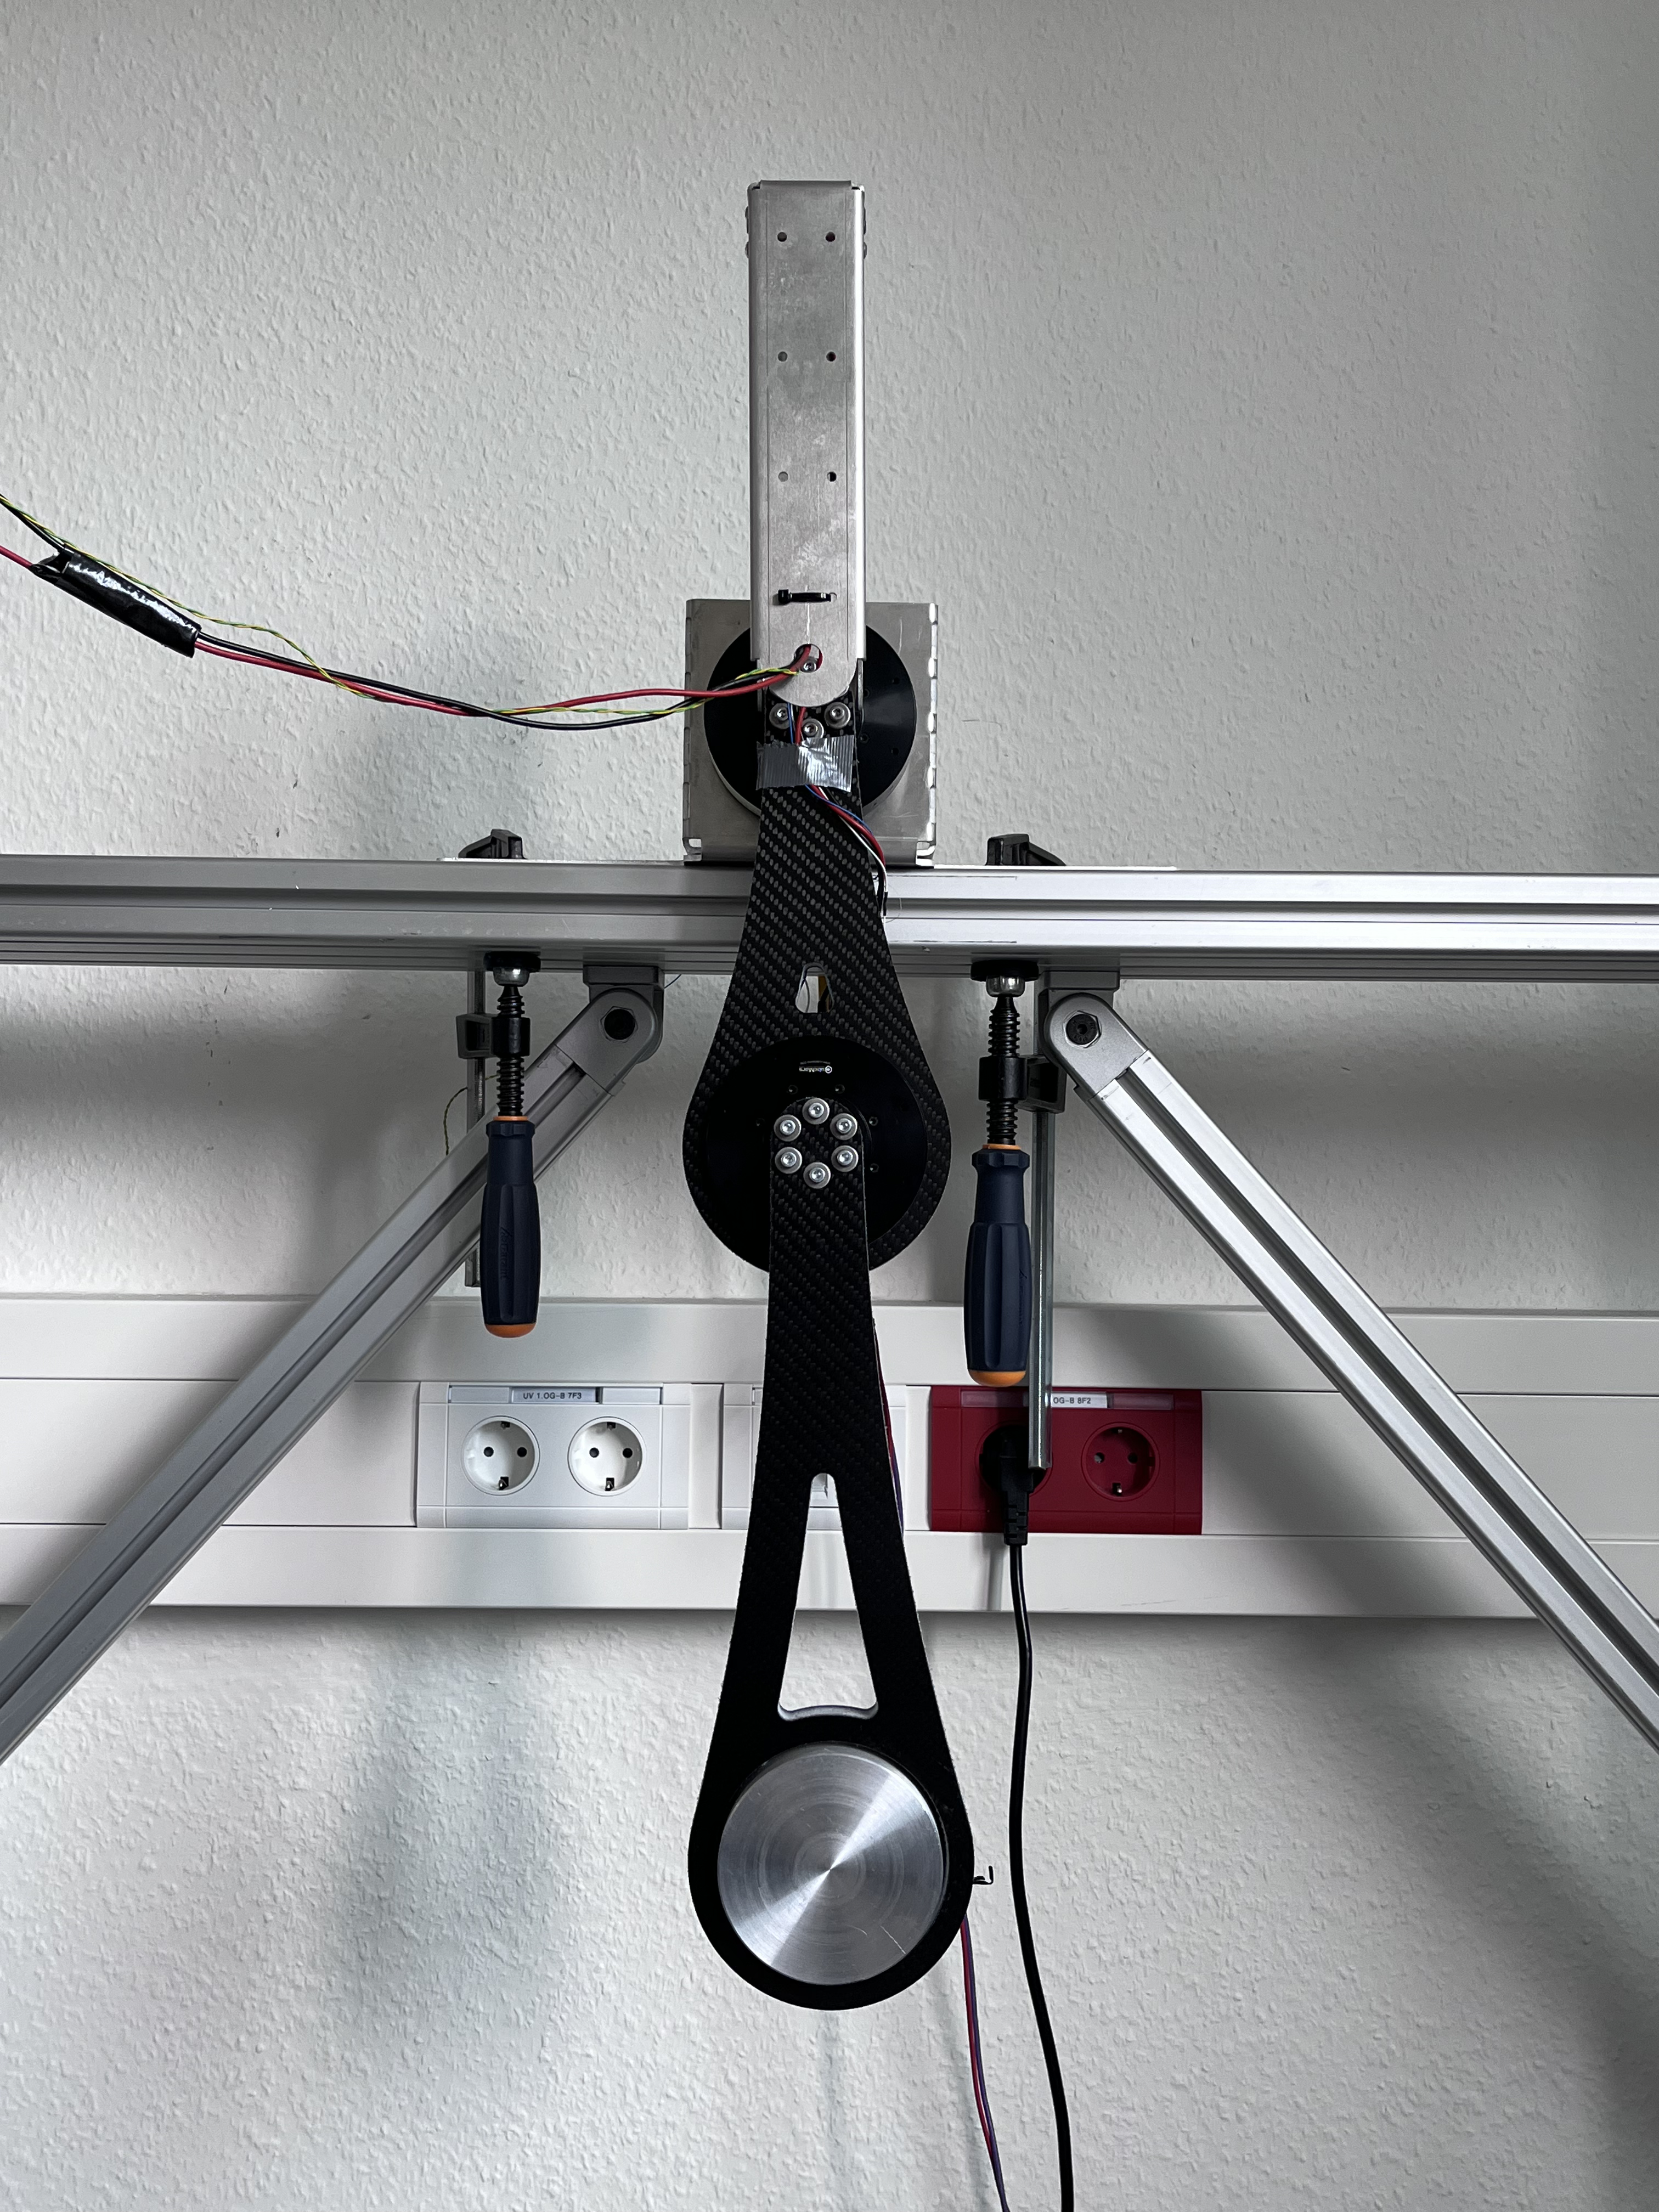
\includegraphics[width=0.45\textwidth]{figures/double_pendulum_real_system.png}
    \caption{Double pendulum in real system}
    \label{fig:image_b}
\end{figure}

The complete real-world test procedure is as follows: power up, manually set the initial state, release the emergency button, run the initialization script (which enables the motor, sets the current position to zero, and tests the CAN connection), confirm the start of the test, record video, draw plots, and exit the test. This procedure is illustrated in the flow chart below:

\begin{figure}[H]
    \centering
    \includegraphics[width=0.9\textwidth]{figures/hardware_setup/testing_procedure.png}% Second image
    \caption{Real hardware system testing procedure}
    \label{fig:image_b}
\end{figure}

Below is an example of one of our successful tests. [some explanation] We executed a sequence of 10 tests to determine the success rate and other key metrics for evaluating performance and robustness. These results will be discussed in the next chapter. 

\begin{figure}[H]
    \centering
    \includegraphics[width=1.1\linewidth]{figures/hardware_result/pendubot_real_system_working.png}
    \caption{Pendubot results on real systems}
    \label{fig:my_label}
\end{figure}


\cleardoublepage
